\chapter[Spectrum Database]{Spectrum Database}
%\addcontentsline{toc}{chapter}{Chapter 3\\Spectrum Database}
\label{chapter:Database}
In Chapter \ref{chapter:Database}, the overview of spectrum sharing with spectrum database and the measurement-based Spectrum Database proposed by our laboratory. And a problem of Spectrum Database Construction is described.

\section{Overview of Spectrum Sharing with Spectrum Database}
For further improving the performance for spectrum sharing, Federal Communications Commission(FCC), an independent agency of the United States government,proposed to fully utilize spectrum database for supporting spectrum sharing. Secondary User should obtain own postion by Global Position System(GPS) and access to database. FCC has already released the detailed rule of construction and managementfor TV broadcasting White Space and some service provider corporation have already established spectrum databases.\cite{ref:fcc,ref:google,ref:microsoft}. However, FCC-defined Database is determined by following a specified propagation model and only stores the decision information whether the White Space can be utilized or not at each position based on the calculation result from the propagation model. Based on the information from GPS, Secondary User accesses to the spectrum database to obtain the White Space information. Because interference towards Primary User is designed by managing geographic White Space conservatively, FCC-defined Spectrum Database is only treated as overlay spectrum sharing. Consequently, as the interference margin is set too large, the calculation of interfernce power with following a detailed propagation model is not considered, which is described in Chapter \ref{chapter:CR} that the spectrum usage efficiency improvement has a upper limit.
\begin{figure}[!htp]
\begin{center}
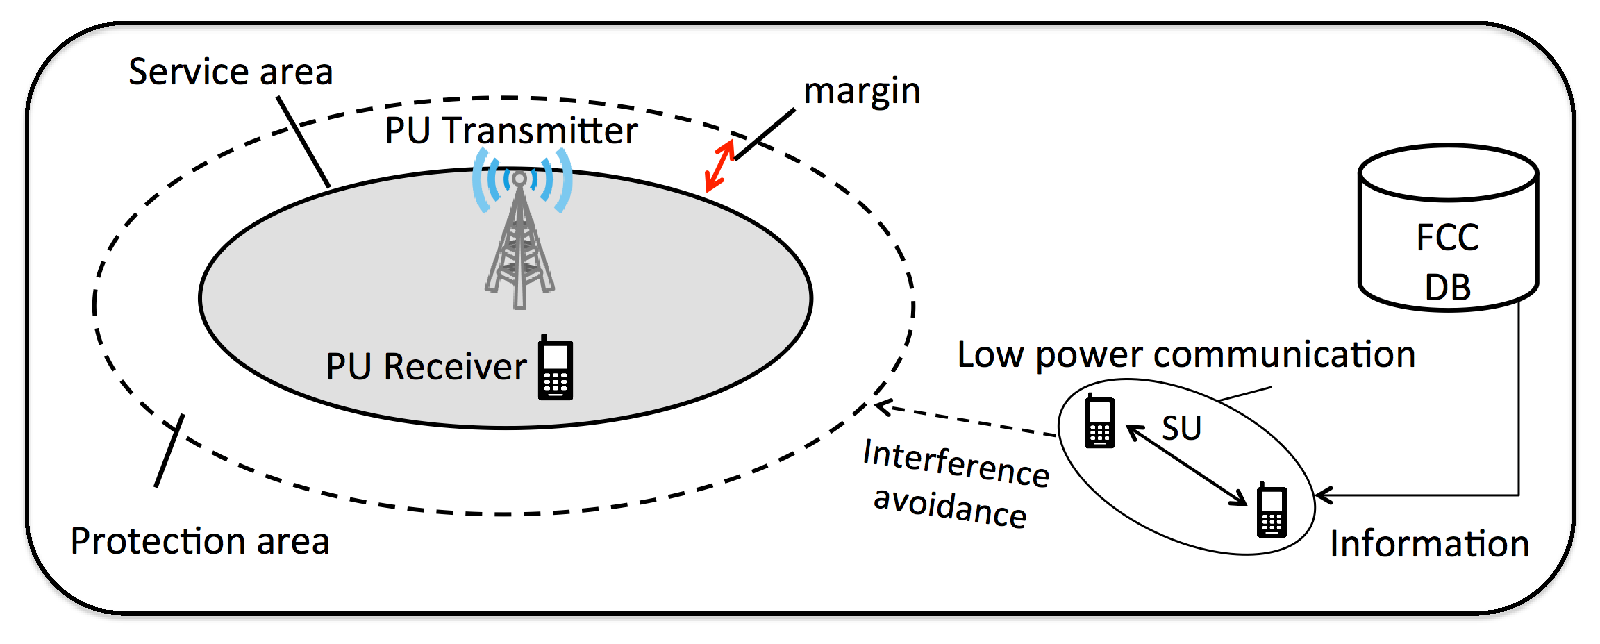
\includegraphics[width=120mm,clip]{fcc_sdb.eps}
\caption{FCC-defined Spectrum Database.}
\label{fig:fcc-defined_sdb}
\end{center}
\end{figure}

\section{Measurement-based Spectrum Database}
To obtain a large improvement on spectrum usage efficiency, underlay spectrum sharing spectrum database should be considered instead of overlay type. Thus, a more advanced radio environment database besides FCC-defined spectrum database is required for providing not only the White Space information, but also the information about Primary, such as Modulation and Coding Scheme(MCS) and transmision power, a more detailed propagation model, estimation error and the position of Primary receiver and so on. As the Spectrum Database is contructed based on the observation on primary signal, high-speed communication is possible to be realized  with adaptively determining the transmission power for avoiding interference towards Primary User based on the information obtained from the underlay spectrum sharing database.

The difference between FCC-defined Spectrum Database and measurement-based Spectrum Database is described as follows and Fig. \ref{fig:fcc-defined_sdb} and \ref{fig:asdb}. In FCC-defined Spectrum Database as illustrated in Fig.\ref{fig:fcc-defined_sdb}, a service area is determined in advance, and the margin level is calculated for protecting Primary User receivers in this service area. Then, the transmission power and service area for Secondary User is limited for avoiding interference towards Primary User. Thus, only low power communication and limited service area is suitable for spectrum sharing. On the other hand, As Measurement-based Spectrum Database is possible to provide all information about Primary User,whiche leads to a more detailed service area, received power from Primary User at each position is known to Secondary User. Therefore, a highly accurate design of transmission power and timing can be realized. As a result, spectrum sharing  performance with Primary User and opportunity for Secondary will be improved and the Quality of Service(Qos) for Secondary User will be enhanced. 

\begin{figure}[!htp]
\begin{center}
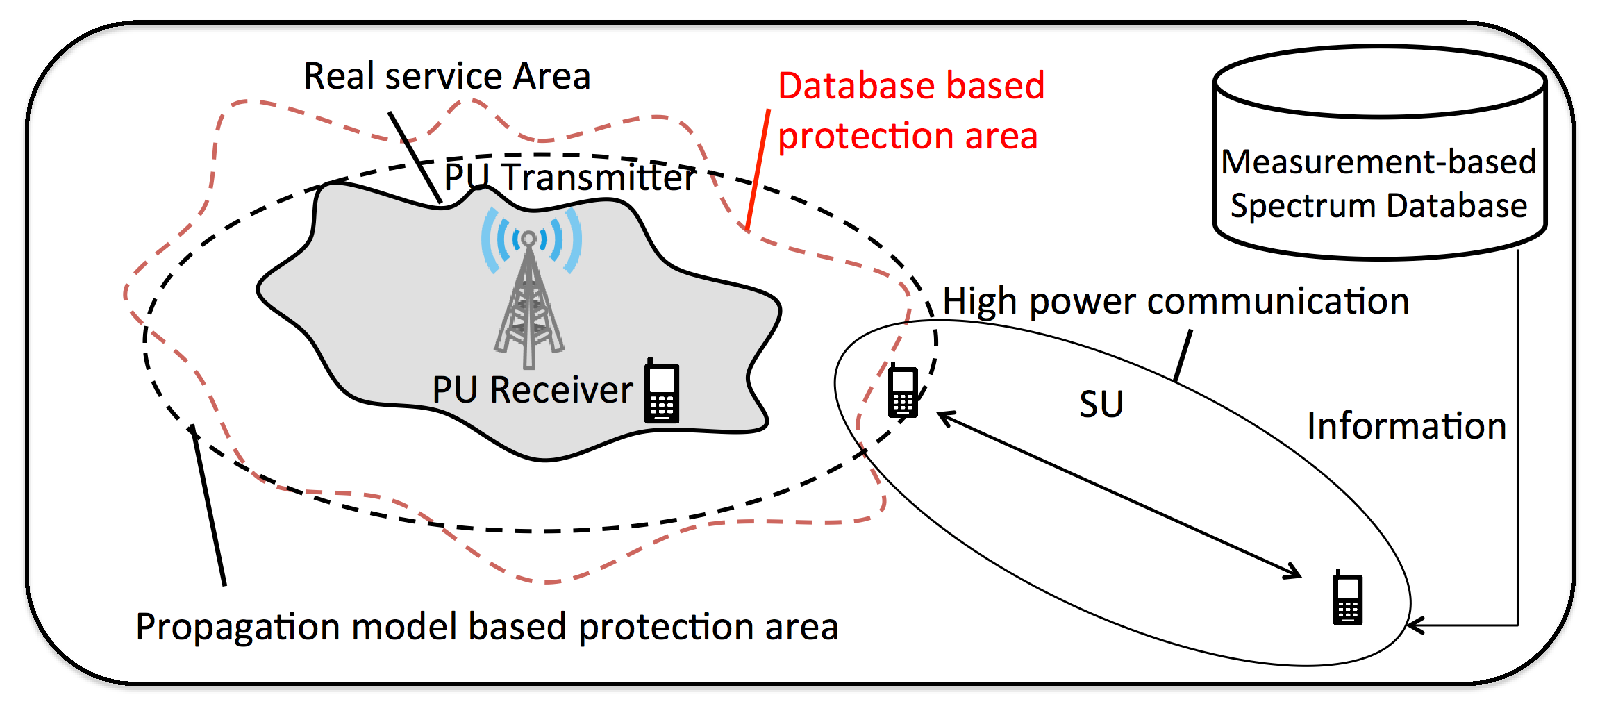
\includegraphics[width=120mm,clip]{asdb.eps}
\caption{Measurement-based Spectrum Database.}
\label{fig:asdb}
\end{center}
\end{figure}

\section{Spectrum Datbase Construction based on Energy Detection}
In this section, the measurement-based spectrum database considered in this research is described in detail. Fig. \ref{fig:fujii_sdb} shows the overview of how to construct the spectrum database. First, the spectrum database stores the radio environment information measured from Secondary User with mobility, such as vehicles and celluar phone. Secondary User receives the signal from Primary User when Secondary User moves without transmitting any signals. After that, Energy Detection(ED)\cite{ref:ED}, a simple and easy to implement spectrum sensing method, is adopted as a measurement method for uploading to the spectrum database. Energy Detection is considered as instantaneous primary signal sampling process during a sensing period $T$, and then $N$ samples is obtained with determining a sampling frequency $F$. As a example, we assume that a series of samples $\left\{x_1,x_2,...,x_N\right\}$are obtained by using energy detection, and then the received power $P$ can be calculated as the following equation

\begin{eqnarray}
P=\frac{1}{N}\sum_{i=1}^{N}(x_i)^2,
\end{eqnarray}

which is only the calculation of the average power of obtained samples.
After Secondaray User finishes observation, the collect measurement will be uploaded to the spectrum database with its own position. Then, a statistical process of estimating the radio environment characterics of Primary User is executed to generate a radio environment map. However, Secondary User, as the source for spectrum database construction, requires highly accurate spectrum sensing performance. If measurment data including error may register to the database, the reliability of spectrum database may degrade. Therefore, the problem of spectrum database construction is explained in the next section.
\section{Problem of Spectrum Database Construction }

